\chapter{کارهای پیشین}
\section{مطالعات بیشتر}

ادبیات در مورد کدگذاری شاخص گسترده و به سرعت در حال رشد است؛ به عنوان مثال، رساله‌های El Rouayheb \lr{[63]} و Blasiak \lr{[30]}، و همچنین یک بررسی اخیر \lr{[33]} را ببینید. در این بخش، ما تعدادی اشاره به موضوعاتی داریم که تاکنون پوشش نداده‌ایم.

\section{12.1 فراتر از \lr{Multiple Unicast}}
در این مونوگراف، ما درخواست‌های \lr{multiple-unicast} پیام‌ها را در نظر گرفتیم، که هر یک از چندین پیام باید دقیقا در یک گیرنده بازیابی شود. در تنظیمات \lr{multiple-groupcast} کلی‌تر، می‌توان بیش از یک گیرنده داشت که همان پیام را درخواست کند. به عنوان مثال، مسئله کدگذاری شاخص \lr{multiple-groupcast} با 3 پیام (1|2)، (1|2, 3)، (2|3)، (3|2) با چهار گیرنده 1a، 1b، 2 و 3 را در نظر بگیرید. هر دو گیرنده 1a و 1b همان پیام \(x_1\) را درخواست می‌کنند، اما با مجموعه‌های متفاوتی از اطلاعات جانبی \(x_2\) و \((x_2, x_3)\)، به ترتیب.
یک نمونه از مسئله کدگذاری شاخص \lr{multiple-groupcast} می‌تواند به طور طبیعی با شناسایی هر گیرنده با یک لبه هایپر مستقیم نشان داده شود؛ برای مثال، (1, \{2\})، (1, \{2, 3\})، (2, \{3\})، و (3, \{2\}) در مثال بالا. این توسعه هایپرگراف از کدگذاری شاخص در \lr{[3]} معرفی شد و بیشتر محدودیت‌های عملکرد و طرح‌های کدگذاری که ما در بخش‌های 5 و 6 بحث کردیم، می‌توانند به راحتی به چنین هایپرگراف‌هایی سازگار شوند؛ به عنوان مثال، \lr{[28]} را برای تعمیم مرز \lr{polymatroidal} برای هایپرگراف‌ها ببینید. نرخ پخش تمام مسائل کدگذاری شاخص \lr{multiple-groupcast} با تا 3 گیرنده در \lr{[149]} مشخص شده است.
در برخی کاربردها، مانند شبکه‌های توزیع محتوا،

هر گیرنده ممکن است علاقه‌مند باشد به دریافت هر پیامی که قبلاً به عنوان اطلاعات جانبی نداشته است. در این مسئله کدگذاری شاخص قابل انعطاف \lr{[31, 138]}، چنین انعطاف‌پذیری می‌تواند مقدار ارتباطات را کاهش دهد - گاهی اوقات به طور قابل توجهی. به عنوان مثال، برای مسئله کدگذاری شاخص قابل انعطاف 3 پیامی \((\ast|2)\)، \((\ast|3)\)، \((\ast|1, 2)\)، نرخ پخش 1 است، که با ارسال \(x_2 + x_3\) حاصل می‌شود، بنابراین \(x_3\) به گیرندگان 1 و 3 منتقل می‌شود، در حالی که \(x_2\) به گیرنده 2 منتقل می‌شود. در مقایسه، مسئله کدگذاری شاخص معمولی (1|2)، (2|3)، (3|1, 2) که با همان مجموعه‌های اطلاعات جانبی سازگار است، نیاز به نرخ پخش 2 دارد. به عنوان یک مثال ساده‌تر، اگر هیچ گیرنده‌ای هیچ اطلاعات جانبی در مورد \(n\) پیام نداشته باشد، کدگذاری شاخص قابل انعطاف اجازه می‌دهد فقط \(x_1\) منتقل شود (β = 1)، در حالی که کدگذاری شاخص معمولی نیاز به انتقال بدون کد \((x_1, . . . , x_n)\) دارد (β = n).
گاهی اوقات اطلاعات جانبی در یک گیرنده دقیقاً مجموعه‌ای از پیام‌های دیگر نیست، بلکه برخی از توابع پیام‌ها (یعنی کدوردها) است که از انتقال‌های گذشته شنیده شده‌اند. این مسئله کدگذاری شاخص با اطلاعات جانبی کدشده در \lr{[50]} مطالعه شد، جایی که هم اطلاعات جانبی در گیرندگان و هم خود درخواست‌ها می‌توانند ترکیبات خطی از پیام‌ها باشند؛ همچنین \lr{[92, 32]} را ببینید.
به عنوان یک تغییر دیگر، اطلاعات جانبی ممکن است به طور همزمان بین سرور و گیرندگان به اشتراک گذاشته نشود. در مسئله کدگذاری شاخص کور \lr{[83]}، سرور نمی‌داند که کدام اطلاعات جانبی در هر گیرنده موجود است، اما مقدار (کدشده) اطلاعات جانبی را می‌داند. در مسئله کدگذاری شاخص با اطلاعات جانبی اشتباهی \lr{[85]}، گیرندگان ممکن است اطلاعات جانبی دقیقی نداشته باشند.


\section{12.2 پخش پر سر و صدا}

یکی از ساده‌سازی‌های بزرگ در مسئله کدگذاری شاخص این است که پیوند پخش بی‌صدا است. با این حال، برای برخی از کاربردهای عملی، این موضوع باید تسهیل شود. یکی از ساده‌ترین نمونه‌های چنین تسهیلی، مشکل کانال پخش تکمیلی \lr{[155, 157, 89]} است که در شکل 12.1 نمایش داده شده است. این مسئله مشکل کدگذاری شاخص 2 پیام (1|2),(2|1) را تعمیم می‌دهد با جایگزینی پیوند پخش بی‌صدا با یک کانال پخش پر سر و صدا \(p(v1, v2|u)\) با ورودی \(U\) و خروجی‌های \(V1\) و \(V2\). همانطور که قبلاً، پیام‌ها \(Xi \in \{0, 1\}^{ti}\)، \(i = 1, 2\) هستند، و نرخ‌های ارتباط بیش از \(r\) استفاده از کانال پخش با کدورد \(Ur\) و مشاهدات پر سر و صدای آن \(V1r\) و \(V2r\) به ترتیب \(t1/r\) و \(t2/r\) هستند. بنابراین، یک کد \((t1,t2,r)\) برای این مشکل تعریف می‌شود توسط رمزگذار \(Ur = \phi(X1,X2)\) و دو رمزگشا \(X̂1 = \psi1(V1r, X2)\) و \(X̂2 = \psi2(V2r, X1)\). تعاریف جفت نرخ قابل دستیابی و منطقه ظرفیت همانند مشکل کدگذاری شاخص بی‌صدا با احتمال میانگین خطای ناچیز ارائه شده در ضمیمه 1.A هستند. منطقه ظرفیت برای این مشکل می‌تواند مشخص شود به عنوان مجموعه بسته محدب شامل تمام جفت نرخ‌ها \((R1, R2)\) که برآورده می‌کنند
\begin{align*}
    R1 &\leq I(U;V1) \\
    R2 &\leq I(U;V2)
\end{align*}

برای برخی \(p(u)\).

مشکل ارتباط بر کانال پخش با اطلاعات جانبی دلخواه گیرنده، که ممکن است به خوبی به عنوان مشکل کدگذاری شاخص پر سر و صدا نامیده شود، به طور کلی بسیار دشوار است، حتی برای تعداد کمی از پیام‌ها. به عنوان مثال، منطقه ظرفیت کانال پخش دو گیرنده استاندارد \lr{[48]} (مطابق با (1|−),(2|−)) هنوز باز است. برای چندین مورد خاص جالب مانند کانال‌های پخش گوسی، با این حال، منطقه ظرفیت می‌تواند شخصیت‌دار شود برای یک جفت گیرنده‌ها \lr{[163, 137, 16]}.

چندین تکنیک کدگذاری برای کدگذاری شاخص پر سر و صدا توسعه داده شده‌اند. کدهای جبری و محدودیت‌های عملکرد آن‌ها برای کدگذاری شاخص در \lr{[52]} مطالعه شده‌اند؛ همچنین \lr{[32]} را ببینید. سایر تکنیک‌های کدگذاری بر اساس مدولاسیون \lr{[112]} و شبکه‌ها \lr{[113, 79]} توسعه داده شده‌اند.
\begin{figure}
    \centering
    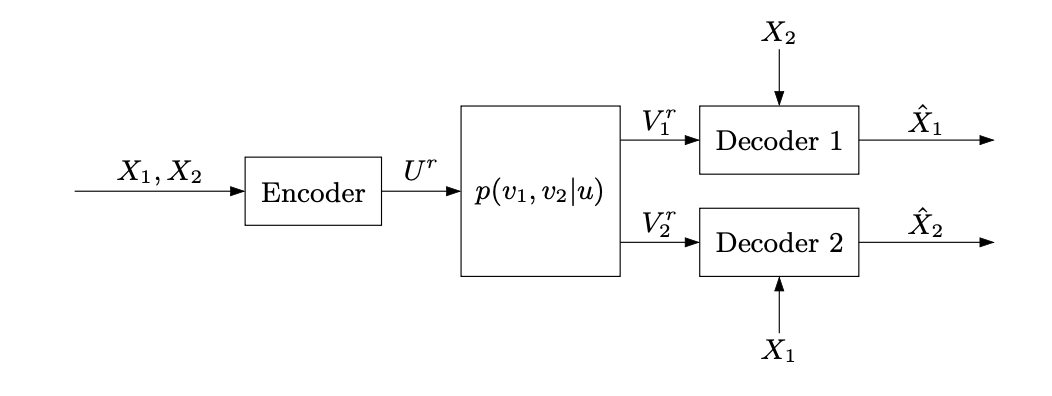
\includegraphics{figs/chapter8/12.1.png}
    \caption{Caption}
    \label{fig:my_label}
\end{figure}
\section{12.3 سرورهای توزیع شده}

در برخی از کاربردها، داده‌ها به طور جغرافیایی توزیع شده و در سراسر بسیاری از مکان‌ها ذخیره می‌شوند. مشکل کدگذاری شاخص توزیع شده، نشان داده شده در شکل 12.2، یک توسعه از مشکل کدگذاری شاخص به چنین سناریوهای ارتباطی است. این مشکل اولین بار در \lr{[116]} مطالعه شد و در \lr{[124]} به 2n − 1 سرورها تعمیم داده شد که هر کدام یک زیرمجموعه غیرخالی از پیام‌ها \(x(J)\)، \(J \subseteq [n]\)، را به کدورد خودشان زیر برخی محدودیت ظرفیت پیوند رمزگذاری می‌کنند.


چندین محدودیت عملکرد و تکنیک‌های کدگذاری برای مشکل کدگذاری شاخص متمرکز که ما در بخش‌های 5 و 6 بحث کردیم، می‌توانند به مورد توزیع شده تعمیم داده شوند \lr{[145, 93, 94, 95]}. به طور خاص، طرح کدگذاری ترکیبی (بهبود یافته) توسعه یافته در بخش 6.10 می‌تواند به طور طبیعی به چندین سرور توسعه داده شود با مطابقت دادن شاخص‌های ترکیبی به سرورهایی که می‌توانند آن‌ها را تولید کنند \lr{[94]} و با ارسال شاخص‌های ترکیبی به صورت همکارانه از طریق آن سرورها \lr{[93]}؛ \lr{[95]} را برای جزئیات ببینید. وقتی با یک مرز بیرونی عمومی که ترکیبی از اصول پلی‌ماترویدال مشابه با آن‌هایی که در مرز پلی‌ماترویدال در بخش 5.2 با تکنیک‌های جداسازی وابستگی عملکردی استفاده شده‌اند \lr{[88, 144]}، جدا می‌شود، این طرح کدگذاری ترکیبی توزیع شده، ظرفیت مجموع برای تمام مشکلات کدگذاری شاخص تا چهار پیام تحت ظرفیت‌های پیوند برابر در \lr{[95]} برقرار شده است.
\begin{figure}
    \centering
    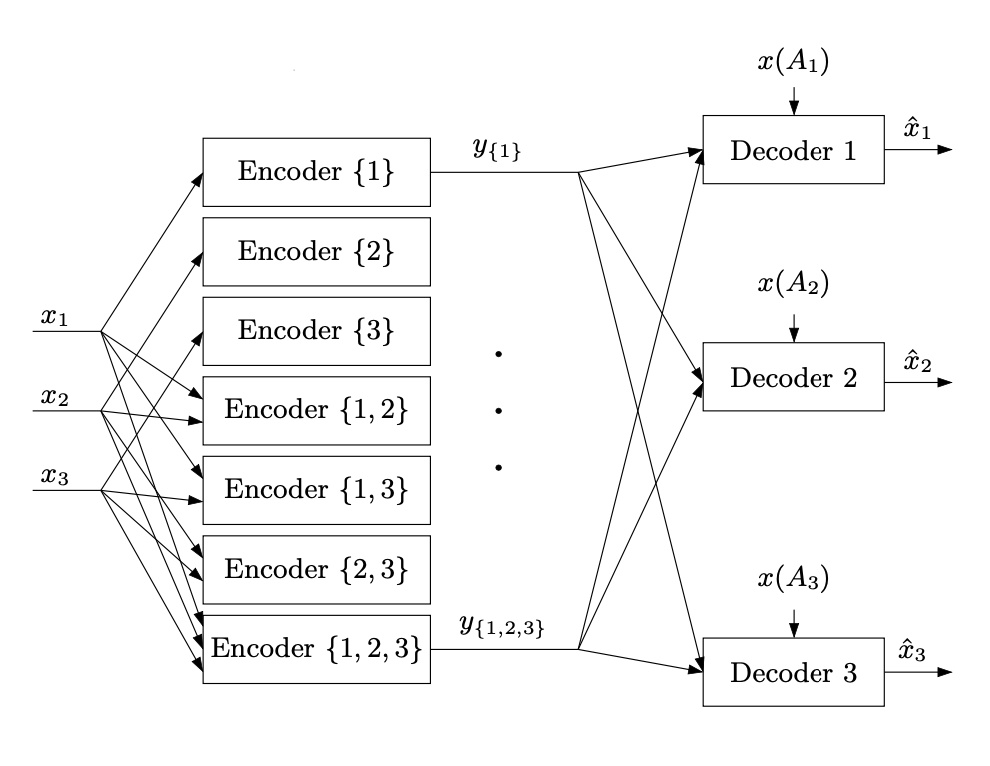
\includegraphics{figs/chapter8/12.2.png}
    \caption{Caption}
    \label{fig:my_label}
\end{figure}

\section{12.4 امنیت و حریم خصوصی}


ارتباط امن در برابر شنودگران مسئله‌ای مهم در بسیاری از شبکه‌های ارتباطی است؛ به عنوان مثال، مقاله بنیادین \lr{[37]} در مورد کدگذاری شبکه امن و توسعه‌های بعدی آن \lr{[36, 38, 136, 64]} را ببینید. یک مسئله کدگذاری شاخص را در نظر بگیرید که در آن یک شنودگر دانش جزئی از پیام‌ها و کدورد پخش را دارد و سرور باید جلوی شنودگر را بگیرد از یادگیری هرگونه اطلاعات در مورد برخی یا تمام پیام‌ها. این مشکل کدگذاری شاخص امن اولین بار در \lr{[51]} در زمینه کدهای خطی اسکالر مطالعه شد و سپس برای کدهای غیرخطی عمومی در \lr{[118]} توسعه یافت. ارتباط بین کدگذاری شبکه امن و کدگذاری شاخص امن (که موازی با رابطه بین نسخه‌های غیرامن بحث شده در بخش 10 است) در \lr{[117]} توسعه یافت.

یکی از فرمول‌بندی‌های معیاری برای کدگذاری شاخص امن، موردی است که در آن شنودگر دسترسی کامل به کدورد پخش و برخی از پیام‌ها دارد و نباید هیچ اطلاعاتی در مورد هیچ پیام تکی (فراتر از اطلاعات جانبی که از قبل دارد) یاد بگیرد. برای این مشکل، طرح‌های کدگذاری تخت و ترکیبی که در بخش 6 بحث شد، می‌تواند به راحتی گسترش داده شود تا ارتباط قابل اطمینان و رازداری ضعیف (یعنی، نرخ نشت اطلاعات ناپدید شونده) را به طور همزمان دستیابی کند \lr{[98]}. وقتی با مرز بیرونی که مرز پلی‌ماترویدال در بخش 5.2 را با نابرابری‌های اضافی بر اساس محدودیت‌های رازداری افزایش می‌دهد مقایسه می‌شود، طرح کدگذاری ترکیبی امن منطقه ظرفیت را برای تمام مشکلات تا سه پیام دستیابی می‌کند \lr{[98]}.

یکی دیگر از فرمول‌بندی‌های معیاری، مشکل کدگذاری شاخص کاملاً امن است، که در آن شنودگر هیچ اطلاعات جانبی اضافی ندارد، اما نباید هیچ اطلاعاتی از هر نوع در مورد پیام‌ها از کدورد پخش (یعنی، صفر اطلاعات متقابل همانند سیستم رازداری شانون \lr{[132]}) یاد بگیرد. این محدودیت رازداری کامل نیاز به یک کلید مشترک بین سرور و گیرنده‌ها دارد. حداقل طول کلید مورد مطالعه و تقریباً در \lr{[110]} مشخص شده است.

گاهی اوقات در سیستم شنودگر مخاصمانه‌ای وجود ندارد، اما ترجیح داده می‌شود که هر پیام فقط برای گیرنده مورد نظر آشکار شود. این مشکل کدگذاری شاخص خصوصی در \lr{[111]} با کدهای خطی مطالعه شده است. نوع دیگری از حریم خصوصی در \lr{[84]} مطالعه شده است، که در آن تقاضا و دسترسی به اطلاعات جانبی هر گیرنده نیز باید از سایر گیرنده‌ها خصوصی نگه داشته شود. کدگذاری شاخص در این زمینه به طور نزدیکی مرتبط با بازیابی اطلاعات خصوصی است \lr{[44, 19]}; \lr{[142]} را برای این اتصال جالب ببینید.



